\documentclass{article}

\usepackage[paper=a4paper,margin=1in]{geometry}
\usepackage[english,spanish]{babel}
\usepackage{multicol}
\usepackage{hhline}
\usepackage{subfig}
\usepackage{amsmath}
\usepackage{amssymb}
\usepackage{graphicx}
\usepackage{cancel}
\usepackage{array}
\usepackage{hyperref}
\usepackage{longtable}
\usepackage[scaled]{helvet}
\renewcommand\familydefault{\sfdefault} 
\usepackage[T1]{fontenc}

\renewcommand{\figurename}{Imagen}

\hypersetup{
    colorlinks=true,
    linkcolor=black,
    filecolor=black,
    urlcolor=blue,
}


\graphicspath{ {./images/} }

\title{Lenguaje Orientado a Objetos - Práctica Final \\ \small Ucel 2023}
\author{Leguina, Damián Adolfo (Legajo 27510)}
\date{2023}

\begin{document}

\maketitle

\tableofcontents

\newpage

\section{Entidades}

Un Usuario tiene un identificador, un nombre, una contraseña, puede ser administrador y puede estar activo.

Un Trabajo tiene un identificador, calidad de copia, cantidad de copias, un estado de progreso, una fecha de inicio de impresión, una fecha de fin de impresión y una fecha de entrega de las impresiones.

Un Usuario puede tener varios Trabajos, un Trabajo le pertenece unicamente a un Usuario.

\begin{figure}[h]
    \centering
    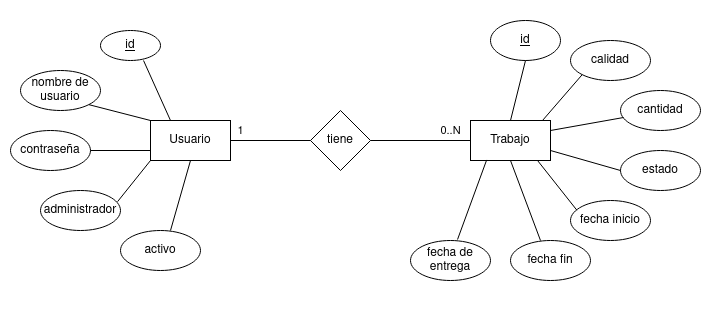
\includegraphics[width=\linewidth,keepaspectratio]{erd.png}
    \caption{Diagrama de entidad-relación.}
\end{figure}

Su representación en tablas relacionales sería

\begin{figure}[h]
    \centering
    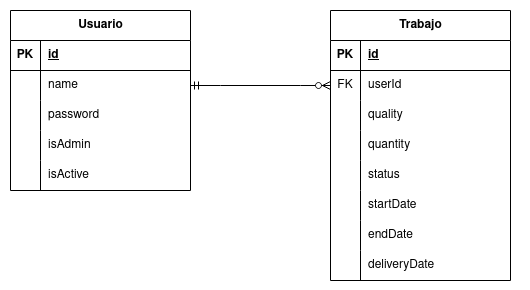
\includegraphics[width=\linewidth,keepaspectratio]{erd-2.png}
\end{figure}

\newpage

\section{Pantallas de la aplicación}

\begin{figure}[h]
    \centering
    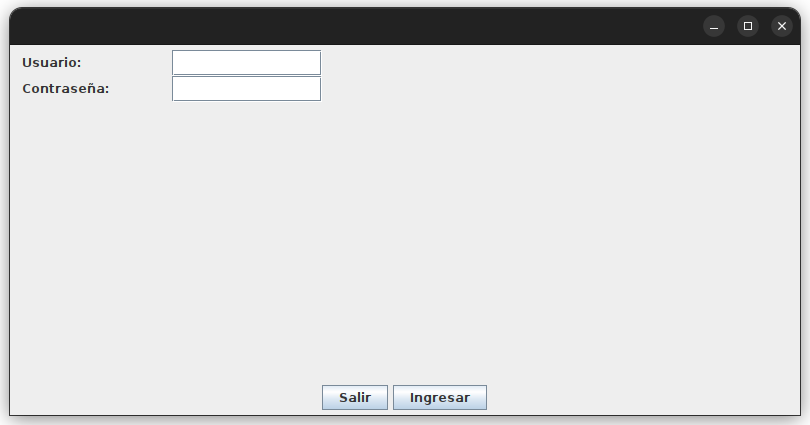
\includegraphics[width=0.7\linewidth,keepaspectratio]{login-frame.png}
    \caption{Pantalla de Login.}
\end{figure}


Ingresar el nombre de usuario en el campo \emph{usuario} y la contraseña en el campo \emph{contraseña} y apretar el botón \emph{Ingresar} para iniciar sesión.

Apretar el botón \emph{Salir} para salir de la aplicación.

\subsubsection*{Posibles problemas}

\begin{itemize}
    \item \emph{``El campo 'Usuario' tiene un valor inválido.''}: El campo \emph{usuario} esta vacío.
    \item \emph{``El campo 'Contraseña' tiene un valor inválido.''}: El campo \emph{contraseña} esta vacío.
    \item \emph{``Usuario no encontrado.''}: El nombre de usuario y/o la contraseña fueron incorrectos.
\end{itemize}

\subsection{Menú}

Pantalla con botones para ir a las funcionalidades específicas de la aplicación, los botones dependen de si el usuario que ingreso es administrador o no.

\begin{figure}[h]
    \centering
    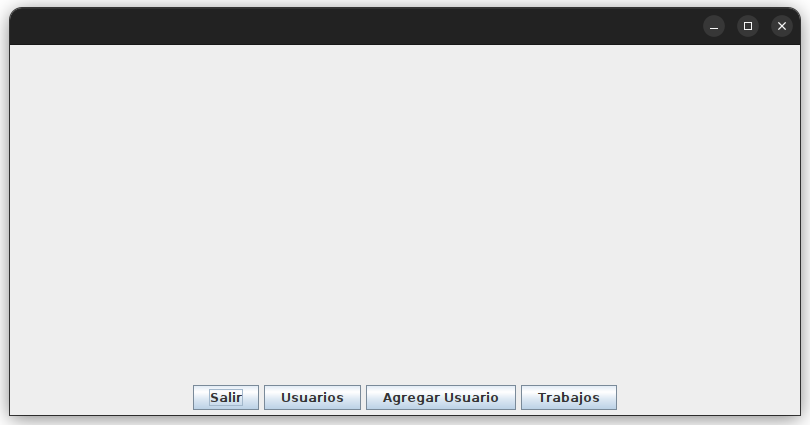
\includegraphics[width=0.7\linewidth,keepaspectratio]{menu-admin.png}
    \caption{Menú de administrador.}
\end{figure}

Para un administrador las opciones son \emph{Usuarios}, lista los usuarios actuales, \emph{Agregar usuario}, lleva a un formulario para dar de alta a un nuevo usuario, y \emph{Trabajos}, lista los trabajos actuales.

\newpage

\begin{figure}[h]
    \centering
    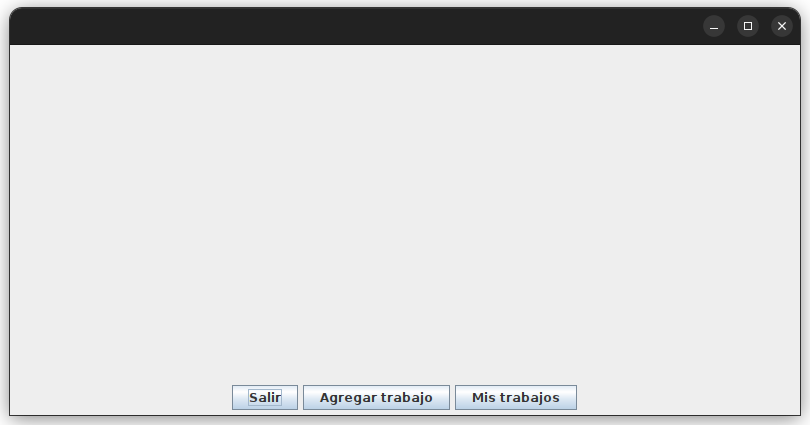
\includegraphics[width=0.7\linewidth,keepaspectratio]{menu-user.png}
    \caption{Menú de usuario.}
\end{figure}

Un usuario no administrador tiene las opciones \emph{Agregar trabajo}, lleva a un formulario para cargar un trabajo nuevo, y \emph{Mis trabajos}, que lista los trabajos del usuario actual.

Los dos tipos de usuario tienen la opción \emph{Salir}, que lleva regresa al menú de login.

\subsection{Usuarios}

Pantalla específica para los administradores.

\begin{figure}[h]
    \centering
    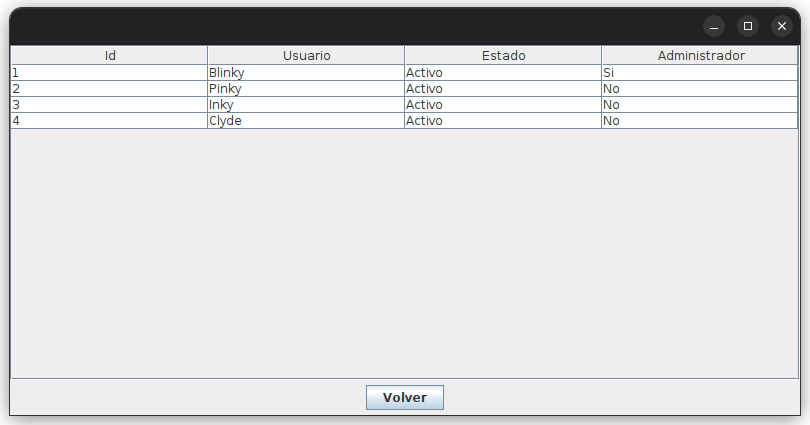
\includegraphics[width=0.7\linewidth,keepaspectratio]{list-users.png}
    \caption{Listado de usuarios.}
\end{figure}

Es una pantalla que lista a los usuarios en una tabla, las filas de la tabla pueden ser seleccionada, y dependiendo de la cantidad de filas seleccionadas botones van a aparecer para realizar diferentes acciones.


En el caso de haber un usuario seleccionado, aparecerán un botón de \emph{Desactivar usuario} o \emph{Activar usuario}, dependiendo de si el usuario este activo o inactivo, apretando este botón se cambiara el estado del usuario seleccionado, y un botón de \emph{Administrar usuario}, que lleva a una pantalla de administración para ese usuario.

\newpage

\begin{figure}[h]
    \centering
    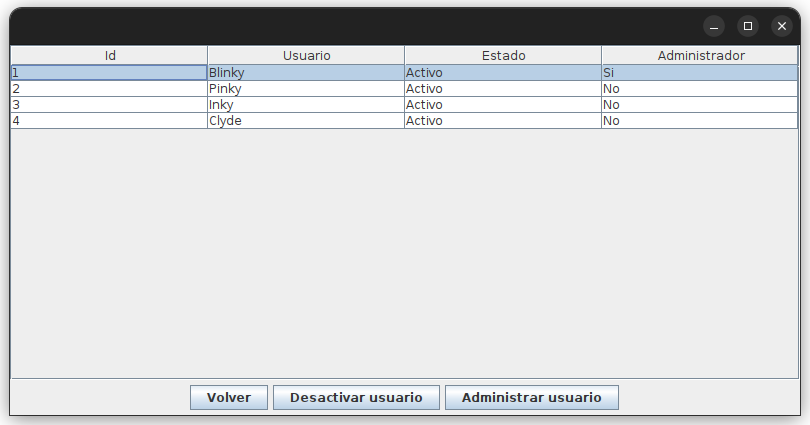
\includegraphics[width=0.7\linewidth,keepaspectratio]{list-users-one-selected.png}
    \caption{Un usuario seleccionado.}
\end{figure}

En caso de haber seleccionado varios usuarios, los botones visibles serán \emph{Desactivar usuarios} y \emph{Activar usuarios}, que desactiva o activa todos los usuarios seleccionados.

\begin{figure}[h]
    \centering
    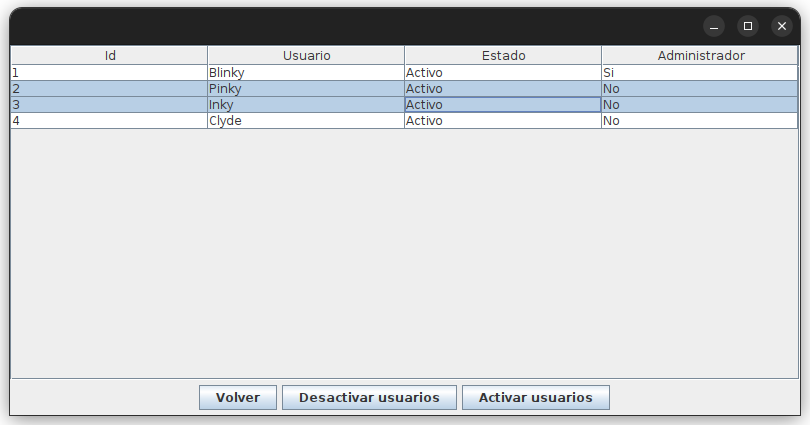
\includegraphics[width=0.7\linewidth,keepaspectratio]{list-users-many-selected.png}
    \caption{Varios usuarios seleccionado.}
\end{figure}
\subsubsection*{Posibles problemas}

\begin{itemize}
    \item \emph{``Un usuario no puede modificar su propio estado.''}: Uno de los usuarios seleccionados es el usuario con el que se ingreso a la aplicación, y ese usuario no puede alterar su propio estado.
\end{itemize}

\newpage

\subsection{Información de Usuario}

\begin{figure}[h]
    \centering
    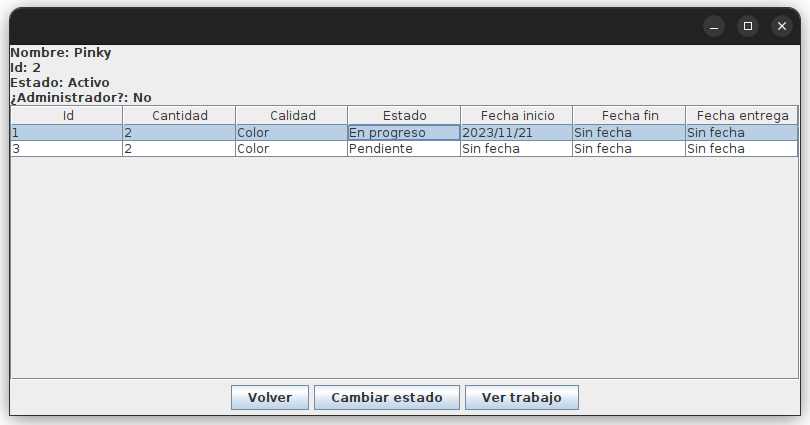
\includegraphics[width=0.7\linewidth,keepaspectratio]{user-info.png}
    \caption{Información de usuario (con un trabajo seleccionado).}
\end{figure}

Pantalla con información pertinente al usuario seleccionado, incluyendo los trabajos pertenecientes a ese usuario. Contiene los botón \emph{Volver}, para volver al listado de usuario.

Si el usuario mostrado en la pantalla es diferente al usuario con el que se ingreso al sistema entonces también habrá un botón \emph{Cambiar estado} que permitirá cambiar el estado del usuario a activo o inactivo

Si el usuario selecciona un trabajo, aparecerá el botón \emph{Ver trabajo}, que lo llevará a una pantalla de información/administración del trabajo seleccionado.

\subsection{Agregar Usuario}

\begin{figure}[h]
    \centering
    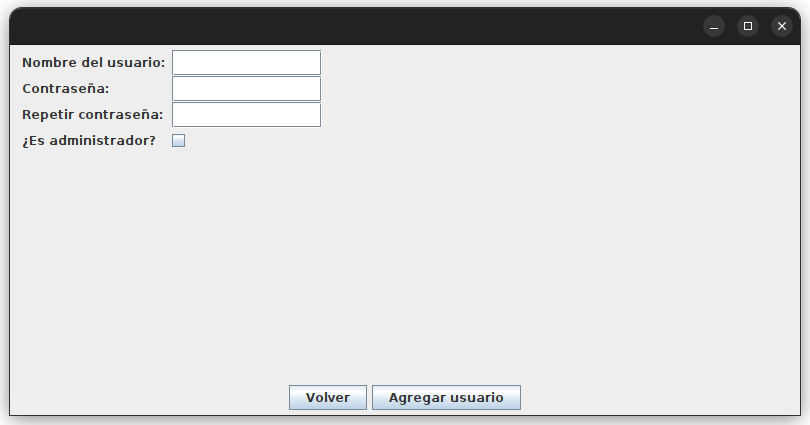
\includegraphics[width=0.7\linewidth,keepaspectratio]{add-user.png}
    \caption{Agregar usuario}
\end{figure}

Pantalla de administrador que permite dar de alta a un usuario nuevo. Contiene un campo \emph{Nombre de usuario} para el nombre, \emph{Contraseña} y \emph{Repetir contraseña} para la contraseña y un checkbox para definir si el usuario nuevo es administrador o no.

\subsubsection*{Posibles problemas}

\begin{itemize}
    \item \emph{``El campo 'Usuario' tiene un valor inválido.''}: El campo \emph{usuario} esta vacío.
    \item \emph{``El campo 'Contraseña' tiene un valor inválido.''}: El campo \emph{contraseña} esta vacío.
    \item \emph{``Las contraseñas no son iguales.''}: Los valores de los campos \emph{Contraseña} y \emph{Repetir contraseña} son diferentes.
    \item \emph{``Ya existe un usuario con ese nombre.''}: Ya hay un usuario cargado con el mismo nombre dado en \emph{Nombre del usuario}.
    \item \emph{``Error al guardar el usuario.''}: La memoria asignada para usuarios esta llena y ya no se pueden agregar más usuarios.
\end{itemize}

\subsection{Agregar Trabajo}

\begin{figure}[h]
    \centering
    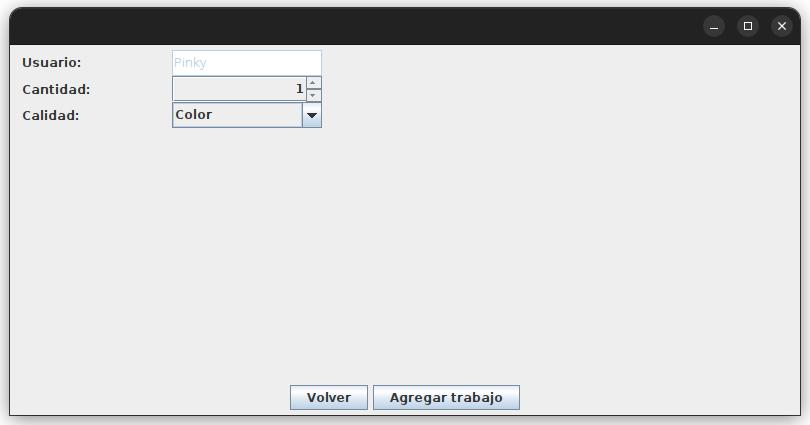
\includegraphics[width=0.7\linewidth,keepaspectratio]{add-print.png}
    \caption{Agregar trabajo}
\end{figure}

Pantalla de usuario no administrador que permite cargar un nuevo trabajo para imprimir. Los campos disponibles son \emph{Cantidad}, la cantidad de copias del trabajo, este valor se tiene que cambiar apretando las flechas del campo o las flechas de arriba y abajo del teclado, no permite ingresar valores con el teclado, y \emph{Calidad}, que puede ``Color'' o ``Blanco y Negro''. El botón \emph{Agregar trabajo} agrega el trabajo y vuelve los campos a los valores por defecto para poder agregar otro trabajo, el botón volver regresa el menú.

\begin{itemize}
    \item \emph{``Error al agregar trabajo.''}: La memoria asignada para trabajos esta llena y ya no se pueden agregar más trabajos.
\end{itemize}

\subsection{Trabajos}

\begin{figure}[h]
    \centering
    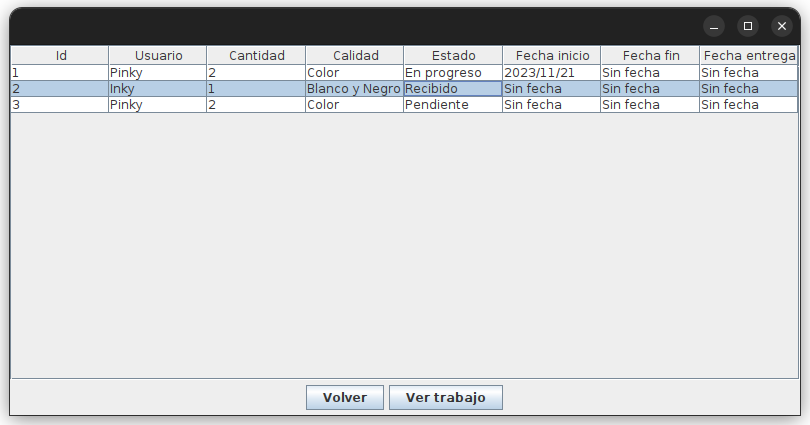
\includegraphics[width=0.7\linewidth,keepaspectratio]{list-prints-admin.png}
    \caption{Listado de trabajos (Administrador)}
\end{figure}

Una pantalla que lista todos los trabajos en caso de que el usuario que ingresa es administrador y los trabajos propios en caso de no ser administrador.

Los botones de acción aparecen dependiendo del tipo de usuario y de la cantidad de trabajos seleccionados, en todo momento, el botón \emph{Volver} esta disponible para regresar al menú principal.

Cuando un administrador selecciona un trabajo aparecerá el botón \emph{Ver trabajo} para ir a una pantalla de información/administración para el trabajo seleccionado.

\begin{figure}[h]
    \centering
    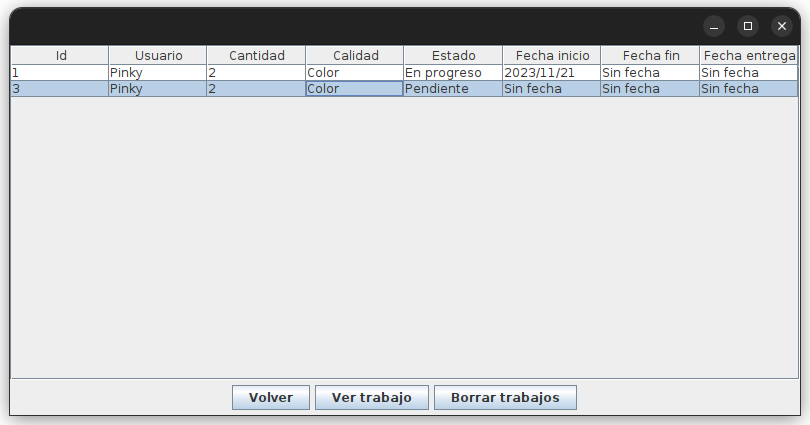
\includegraphics[width=0.7\linewidth,keepaspectratio]{list-prints-user.png}
    \caption{Listado de trabajos (No administrador)}
\end{figure}

Cuando un usuario no administrador selecciona un trabajo, aparecerá el botón \emph{Ver trabajo} para ir a un pantalla de información del trabajo seleccionado, y si el trabajo seleccionado esta en estado ``Pendiente'', aparecerá el botón \emph{Borrar trabajo} para poder eliminarlo.

Cuando un usuario no administrador selecciona varios trabajos, aparecerá el botón \emph{Borrar trabajos}, que permite eliminar todos los trabajos seleccionados, pero si alguno de los trabajos seleccionados no esta pendiente se abortará la operación.

\subsubsection*{Posibles problemas}

\begin{itemize}
    \item \emph{``Uno de los trabajos ya ha comenzado el proceso de impresión.''}: Uno o más de los trabajos seleccionados para borrar esta en un estado diferente a ``Pendiente''.
\end{itemize}

\subsection{Información de trabajo}

\begin{figure}[h]
    \centering
    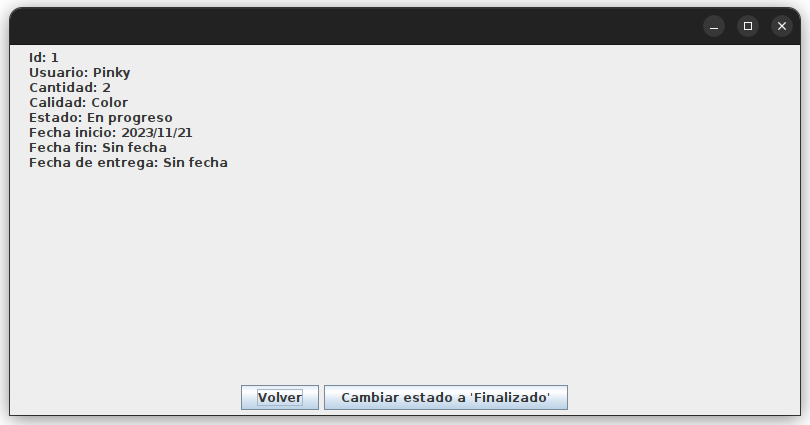
\includegraphics[width=0.7\linewidth,keepaspectratio]{print-info.png}
    \caption{Información de un trabajo (administrador)}
\end{figure}

Pantalla con la información de un trabajo seleccionado, si el usuario mirando la información del trabajo es administrador y el trabajo no esta en estado ``Entregado'', la pantalla va a tener un botón \emph{Cambiar estado} que llevará al trabajo al estado siguiente y actualizara las fechas de ser necesario.

El camino de progreso de un trabajo es ``Pendiente'' $\rightarrow$ ``Recibido'' $\rightarrow$ ``En progreso'' $\rightarrow$ ``Finalizado'' $\rightarrow$ ``Entregado''

Apretando el botón \emph{Volver} se volverá al listado de trabajos o a la pantalla de información de usuario dependiendo de donde se haya ingresado a esta pantalla.

\newpage

\section{Flujo de la aplicación}

\subsubsection*{Máquina de estado de un administrador}
\begin{figure}[h]
    \centering
    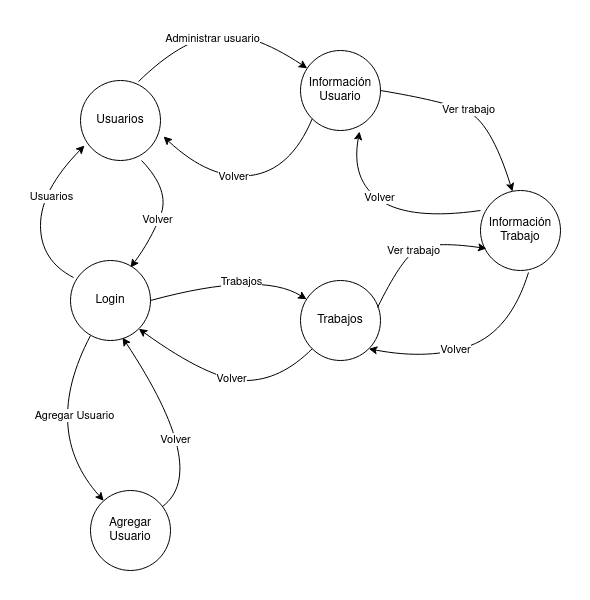
\includegraphics[width=0.7\linewidth,keepaspectratio]{admin-state-machine.png}
\end{figure}

\subsubsection*{Máquina de estado de un usuario no administrador}
\begin{figure}[h]
    \centering
    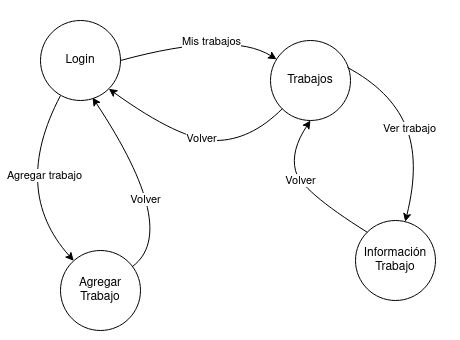
\includegraphics[width=0.6\linewidth,keepaspectratio]{user-state-machine.png}
\end{figure}
\end{document}